In this final section we present a formal specification of some of the requirements explained before.
\begin{lstlisting}[frame = single]
open util/ordering[DateTime]

sig DateTime{}

// some actors in the system
abstract sig User {}

//We don't consider dangling elements 
sig Email{}{
	this in EVD.email
}
sig Password{}{
	this in EVD.password
}
sig Location{}{
	this in ChargingStation.location
}
sig History{
}{
	this in EVD.chargingHistory
}

sig EVD {
	evs: some EV,
    email: one Email, 
	password: one Password,
	chargingHistory: one History
}

sig DSO {}{
	this in ChargingStation.dso
}

abstract sig Socket {}
one sig Type1, Type2, Chademo extends Socket{}

sig EV {
	socket: one Socket,
}{
	this in EVD.evs
}

sig ChargingPoint {
 	socket: some Socket,
	connectedEV: lone EV
}{
	EV.socket in socket
	this in ChargingStation.chargingPoints
}

sig ChargingStation {
	chargingPoints: some ChargingPoint,
	location: one Location,
	dso: one DSO
}{
	this in CPO.chargingStations
}

sig CPO extends User{
	chargingStations: some ChargingStation
}

sig Booking {
	ev: EV,
	cs: ChargingStation,
	cp: ChargingPoint,
	start: DateTime,
	end: DateTime
}{
	// Only Registerd User can book
	ev in EVD.evs &&
	cp in cs.chargingPoints
	lt[start, end]
}

/*********** FACTS  *************/

fact eachChargingToOnlyOneChargingStation{
	all disj x, y : ChargingStation |
		 #(x.chargingPoints & y.chargingPoints) = 0
}

fact eachCStoOnlyOneCPO{
	all disj x, y : CPO |
		 #(x.chargingStations & y.chargingStations) = 0
}

fact eachEVtoOnlyOneEVD {
	all disj x, y : EVD |
		 #(x.evs & y.evs) = 0
}

fact eachEVConnectedToOneChargingPoint{
    all disj x, y: ChargingPoint |
		 #(x.connectedEV & y.connectedEV) = 0
}

// impose that there must not exist multiple bookings for the same vehicles at the same time
fact noEVOverBooking{
	no disj b1, b2: Booking
	| b1.ev = b2.ev && 
 		(gte[b1.start, b2.start] && lte[b1.start, b2.end] ||
 		 gte[b1.end, b2.start] && lte[b1.end, b2.end])
}

// impose that there must not exist multiple bookings for the same charging point at the same time
fact noOverBooking{
	no disj b1, b2: Booking
	| b1.cp = b2.cp && 
		(gte[b1.start, b2.start] && lte[b1.start, b2.end] ||
		 gte[b1.end, b2.start] && lte[b1.end, b2.end])
}

//Only an EV can be in charge for EVD
fact onlyAnEVisChargingForEVD{
	all evd: EVD, disj ev1, ev2 :EV |
	ev1 in evd.evs and ev2 in evd.evs and ev1 in ChargingPoint.connectedEV
	implies ev2 not in ChargingPoint.connectedEV
}

//Unique email to EVD
fact uniqueEmail{
 no disj driver1, driver2: EVD |
 	 driver1.email = driver2.email 
}

//Unique history to EVD
fact uniqueHistory{
 no disj driver1, driver2: EVD |
 	 driver1.chargingHistory = driver2.chargingHistory
}

//Unique location to ChargingStation
fact uniqueLocation{
 no disj cs1, cs2: ChargingStation |
 	 cs1.location = cs2.location
}

/**** ASSERTIONS ****/
// The same charging point can't be in two different charging stations
assert noCPinTwoChargingStations{
	no cp: ChargingPoint, disj cs1, cs2: ChargingStation | 
		cp in cs1.chargingPoints && cp in cs2.chargingPoints
}

assert NoCSInTwoCPO{
 no cs: ChargingStation, disj CPO1, CPO2: CPO |
	cs in CPO1.chargingStations && cs in CPO2.chargingStations
}

assert notExistsCPnotInCS{
	no cp: ChargingPoint
	| cp not in ChargingStation.chargingPoints
}

assert existsEVnotInEVD{
	some ev: EV
	| ev not in EVD.evs
}

assert noBookingForUnEVD{
	Booking.ev in EVD.evs
}

assert noEVOverBooking{
	no disj b1, b2: Booking |
	b1.ev = b2.ev && gte[b1.start, b2.start] && lte[b1.start, b2.end]
}

assert bookingStartLessThanBookingEnd{
	all b: Booking | lt[b.start, b.end]
}

check noCPinTwoChargingStations

check NoCSInTwoCPO

/*********PREDICATES*********/
pred findBookings{
	some disj b1, b2: Booking | lt[b2.end, b1.start]
}

pred addEVToEVD[evd', evd: EVD, NewEv: EV]{
	evd'.evs = evd.evs + NewEv
}
run addEVToEVD

pred addCSToCPO[cpo', cpo: CPO, NewCS: ChargingStation]{
    cpo'.chargingStations = cpo.chargingStations + NewCS
}

run addCSToCPO

pred deleteCSFromCPO[cpo', cpo: CPO, cs: ChargingStation]{
    cpo'.chargingStations = cpo.chargingStations - cs
}

run deleteCSFromCPO

pred addCPToCS
 [cs', cs: ChargingStation, cp: ChargingPoint, cpo: CPO]{
	cs in cpo.chargingStations
	and
	cs'.chargingPoints = cs.chargingPoints + cp 
	implies cpo.chargingStations = cs'
}

run addCPToCS for 20 but exactly 5 ChargingPoint

run findBookings for 10

//To show the CPO interaction with the system
pred CPOworld{
	#CPO >= 2
	#ChargingStation >= 2
	#ChargingPoint >= 5
}

run CPOworld for 20

//To show the EVD interaction with the system
pred EVDworld{
	#EVD >= 2
	#EV >= 4
	#ChargingPoint >= 3
	#ChargingStation >= 2
}

run EVDworld for 10

run {} 
\end{lstlisting}

%TODO: a little explanation for each world important elements
\subsection{Resulting worlds}
\paragraph{The world mainly from the CPO point of view}
From the CPO point of view we show the following world generated with the Alloy analyzer, noticing some important requirements of the eMall:
\begin{itemize}
    \item The CPO manages one or more charging stations
    \item The charging stations have one ore more charging points
    \item The charging points can have different socket types (in the following representation Alloy generated a case in which each charging point has only a socket of one type, but in general the charging point can have many sockets of different types, but we assume that only one is used at the time)
    %TODO: add assumption only a socket is used at the time
    \item The charging stations acquire energy from different DSOs chosen by the CPO, and different charging stations, even of different CPOs, can acquire energy from the same DSO 
\end{itemize}
We can see a simple representation of these elements in the CPOworld:
\begin{figure}[H]
    \centering
    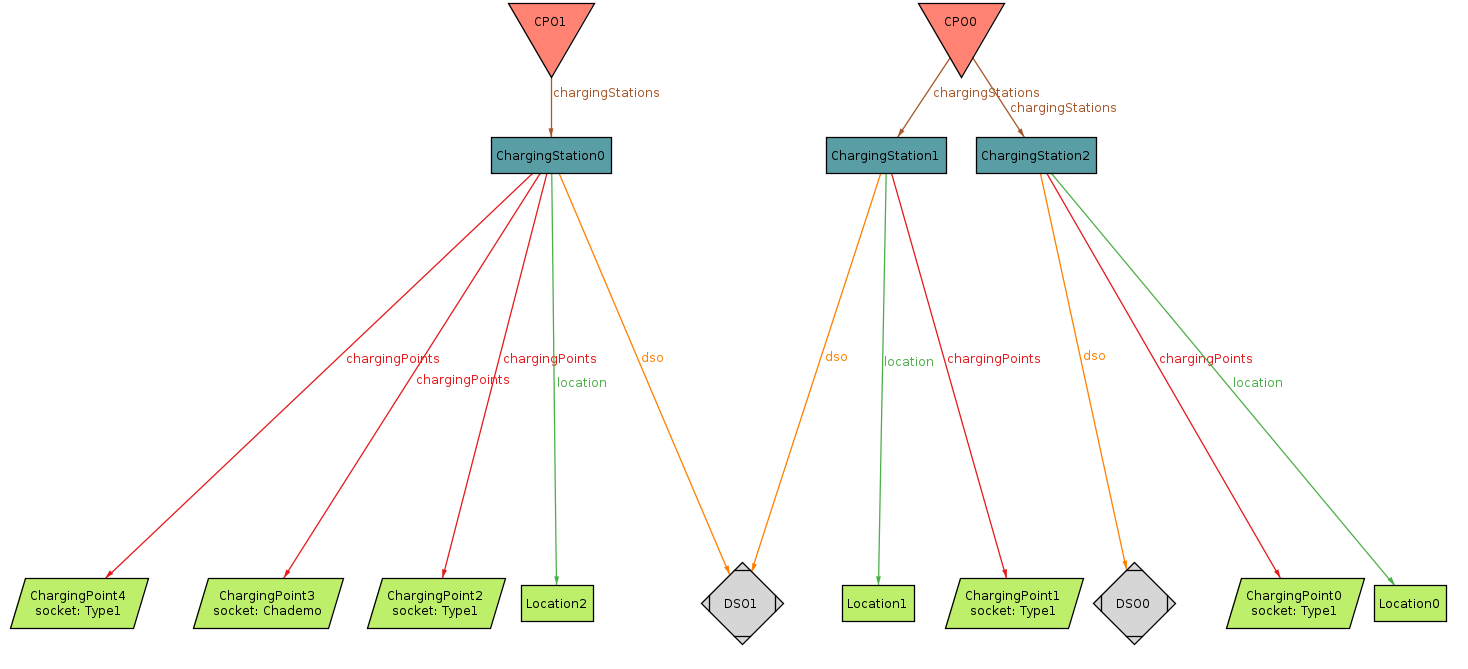
\includegraphics[width=1\textwidth]{Images/cp4/CPOWorld.png}
    \caption{CPOworld}
\end{figure}

%TODO: retake this picture because has RegEVD instead of EVD and see if there are better representations, more focused on the EVD, we have no bookings here, and explain the requirements
\paragraph{The world mainly from the EVD point of view}
To represent the EVD point of view we show another world generated by the Alloy analyzer, in order to verify some requirements: 
\begin{itemize}
    \item The 
\end{itemize}
\begin{figure}[H]
    \centering
    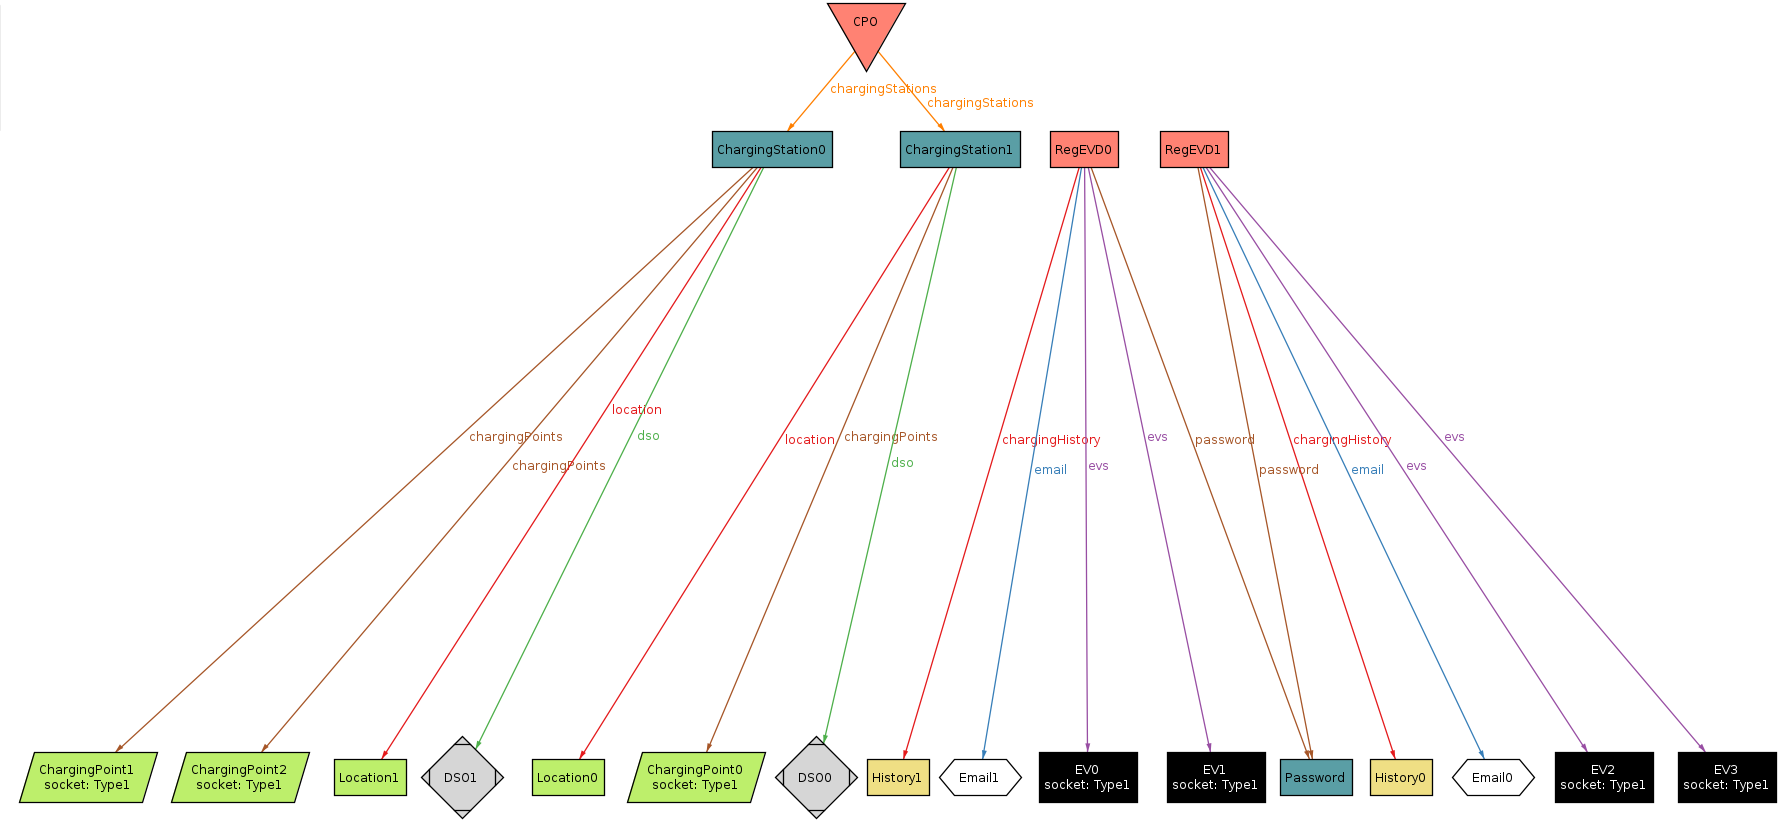
\includegraphics[width=1\textwidth]{Images/cp4/EVDWorldAndCPO.png}
    \caption{EVDworld}
\end{figure}

